% arara: pdflatex
% arara: bibtex
% arara: bibtex
% arara: pdflatex
% arara: pdflatex

\documentclass{dcthesis}

%This version of the thesis template has been updated for the February 2017 thesis guidelines provided by the School of Graduate and Advanced Studies by David Freund and Daryl DeFord.

%  Some good options are draft and singlespacing, for drafts, and *final*,
%for the final cut, and noheadings, for a printout without headings.  
%You can also use the copyright option to add a copyright.  Note:
%final will enforce a bunch of different options, like oneside, 12pt
%and doublespacing, as well as make the margins correct.   Draft, has
%larger margins and is appropriate for two sided printing.   


%%%%%%%%%%%%%%%%%%%%%%%%%%%
%%%%    IMPORTANT     %%%%%
%%%%%%%%%%%%%%%%%%%%%%%%%%%
%
%  Because dvips doesn't know/care about the page size of the dvi file
%  its working on, and because its so important that the margins of
%  your thesis are correct you have to make sure that you are using
%  the command dvi -t letter *thesisnamehere*
%
%  If you are using a terminal this is straightforward, but if you are
%  using a tex editing program it make take a little bit of searching
%  before you figure out how to make this work. 
%  
%  Alternatively, you might consider compiling using pdflatex, which
%  compiles straight to a PDF and doesn't have this problem.  

%%%%%%%%%%%%%%%%%%%%%%%%%%%%%%%%%%%%%%%%%%%%%%%%%%
% Some Defaults
%%%%%%%%%%%%%%%%%%%%%%%%%%%%%%%%%%%%%%%%%%%%%%%%%%
\committee[F. Jon Kull, Ph.D.]{}{}{}{}
\school{Dartmouth College}{Hanover, New Hampshire}
\degree{Doctor of Philosophy}
\field{Mathematics}

%%%%%%%%%%%%%%%%%%%%%%%%%%%%%%%%%%%%%%%%%%%%%%%%%%
% Additional Packages (add as desired)
%%%%%%%%%%%%%%%%%%%%%%%%%%%%%%%%%%%%%%%%%%%%%%%%%%
\usepackage{amsmath,amssymb,amsthm,amsxtra}
\usepackage{mathrsfs} 
\usepackage{lipsum}
\usepackage{xcolor}
\usepackage{hyperref}
\hypersetup{colorlinks=true,urlcolor=blue,citecolor=blue,linkcolor=blue}
\usepackage{tikz}
\usepackage{colonequals}
\usetikzlibrary{arrows,calc,automata,shadows,backgrounds,positioning,intersections,fadings,decorations.pathreplacing,shapes,snakes, matrix}
\usepackage{tikz-cd}
\tikzset{commutative diagrams/.cd, arrow style = tikz, diagrams = {>=latex}}
\tikzset{>=latex}

%\usepackage{index} %Uncomment if you would like to have an index. Compiling with an index takes more work than compiling without one. You will have to look up how to use the index package.

%%%%%%%%%%%%%%%%%%%%%%%%%%%%%%%%%%%%%%%%%%%%%%%%%%
%Formatting
%%%%%%%%%%%%%%%%%%%%%%%%%%%%%%%%%%%%%%%%%%%%%%%%%%
%  Change or add to as desired. 
%  These two commands make the first enumerations look like (a)
%  And the second level like (i).  
% \renewcommand{\labelenumi}{(\alph{enumi})}
% \renewcommand{\labelenumii}{(\roman{enumii})}
%  These commands make the section headings Boldface and not all
%  caps. It also removes the chapter numbers  
\renewcommand{\chaptermark}[1]{\markboth{{\sc #1}}{{\sc #1}}}
\renewcommand{\sectionmark}[1]{\markright{{\sc \thesection\ #1}}}
%  These commands have lowercase headings with chapter numbers. 
%\renewcommand{\chaptermark}[1]{markboth{#1}{}}
%\renewcommand{\sectionmark}[1]{\markright{\thesection\ #1}} 
\newcommand{\PP}{\mathbb P}
\newcommand{\CC}{\mathbb C}
\newcommand{\QQ}{\mathbb Q}
\newcommand{\ZZ}{\mathbb Z}
\renewcommand{\AA}{\mathbb A}
\newcommand{\defi}[1]{\textsf{#1}}
\newcommand{\jv}[1]{{\color{red} \sf JV: [#1]}}
\newcommand{\mm}[1]{{\color{blue} \sf MM: [#1]}}
\newcommand{\wt}[1]{\widetilde{#1}}
\newcommand{\QQal}{{\mathbb Q}^{\textup{al}}}
\newcommand{\QQab}{{\mathbb Q}^{\textup{ab}}}
\newcommand{\QQbar}{{\mathbb Q}^{\textup{al}}}
\newcommand{\kbar}{\overline{k}}
\newcommand{\Kbar}{\overline{K}}
\newcommand{\LL}{\mathscr L}

\DeclareMathOperator{\Div}{Div}
\DeclareMathOperator{\ddiv}{div}
\DeclareMathOperator{\sat}{sat}
\DeclareMathOperator{\ddeg}{deg}
\DeclareMathOperator{\ddim}{dim}
\DeclareMathOperator{\Lifts}{Lifts}
\DeclareMathOperator{\order}{order}
\DeclareMathOperator{\Aut}{Aut}
\DeclareMathOperator{\PGL}{PGL}
\DeclareMathOperator{\Mon}{Mon}
\DeclareMathOperator{\Gal}{Gal}

%%%%%%%%%%%%%%%%%%%%%%%%%%%%%%%%%%%%%%%%%%%%%%%%%%
% Theorem Declarations
%%%%%%%%%%%%%%%%%%%%%%%%%%%%%%%%%%%%%%%%%%%%%%%%%%
% A basic set of theorem declarations.  Add or remove as desired. 
% \newtheorem{prop}{Proposition}[chapter]
\newtheorem{prop}{Proposition}[section]
\newtheorem{theorem}[prop]{Theorem}
\newtheorem{conj}[prop]{Conjecture}
\newtheorem{lemma}[prop]{Lemma}
\newtheorem{corr}[prop]{Corollary}
\theoremstyle{definition}
\newtheorem{definition}[prop]{Definition}
\newtheorem{alg}[prop]{Algorithm}
\newtheorem{notation}[prop]{Notation}
\theoremstyle{remark}
\newtheorem{remark}[prop]{Remark}
\newtheorem{example}[prop]{Example}
\newtheorem*{claim}{Claim}
% numberwithin section for equations and figures
\numberwithin{equation}{section}
\numberwithin{figure}{section}
% \renewcommand{\thefigure}{\arabic{figure}}

%%%%%%%%%%%%%%%%%%%%%%%%%%%%%%%%%%%%%%%%%%%%%%%%%%
%Indices
%%%%%%%%%%%%%%%%%%%%%%%%%%%%%%%%%%%%%%%%%%%%%%%%%%
%This is for an index.  More work is needed for a notation index
%\makeindex

%%%%%%%%%%%%%%%%%%%%%%%%%%%%%%%%%%%%%%%%%%%%%%%%%%
% Macros
%%%%%%%%%%%%%%%%%%%%%%%%%%%%%%%%%%%%%%%%%%%%%%%%%%
% Add your math macros here

%%%%%%%%%%%%%%%%%%%%%%%%%%%%%%%%%%%%%%%%%%%%%%%%%%
% Title Page Information
%%%%%%%%%%%%%%%%%%%%%%%%%%%%%%%%%%%%%%%%%%%%%%%%%%
%  Your personal info goes here!
\title{2-Group Belyi Maps}
\author{Michael James Musty}
\date{\today}
\field{Mathematics}
\degree{Doctor of Philosophy}
%As an optional argument to \committee you can specify the dean of graduate studies.
\committee{John Voight}{Thomas Shemanske}{David Roberts}{Carl Pomerance}

\begin{document}

%%%%%%%%%%%%%%%%%%%%%%%%%%%%%%%%%%%%%%%%%%%%%%%%%%
%Front end of thesis
%%%%%%%%%%%%%%%%%%%%%%%%%%%%%%%%%%%%%%%%%%%%%%%%%%
\frontmatter

\maketitle

%%%%%%%%%%%%%%%%%%%%%%%%%%%%%%%%%%%%%%%%%%%%%%%%%%
%Abstract
%%%%%%%%%%%%%%%%%%%%%%%%%%%%%%%%%%%%%%%%%%%%%%%%%%
%NOTE:  Must be less than 350 words.  
\chapter*{Abstract}
%This is so the abstract appears in the ToC
\addcontentsline{toc}{section}{Abstract}
Write your abstract here.

\chapter*{Preface}
\addcontentsline{toc}{section}{Preface}
Preface and Acknowledgments go here!

%%%%%%%%%%%%%%%%%%%%%%%%%%%%%%%%%%%%%%%%%%%%%%%%%%
%Table of Contents
%%%%%%%%%%%%%%%%%%%%%%%%%%%%%%%%%%%%%%%%%%%%%%%%%%
\tableofcontents

%Add a list of tables
\listoftables

%Add a list of figures
\listoffigures

%%%%%%%%%%%%%%%%%%%%%%%%%%%%%%%%%%%%%%%%%%%%%%%%%%
%Main Portion of Thesis
%%%%%%%%%%%%%%%%%%%%%%%%%%%%%%%%%%%%%%%%%%%%%%%%%%
\mainmatter

%%%%%%%%%%%%%%%%%%%%%%%%%
%%  YOUR THESIS HERE!  %%
%%%%%%%%%%%%%%%%%%%%%%%%%

% \include{chapter1}

\chapter{Introduction}{\label{chapter:intro}
  \section{Belyi maps from a historical perspective}{
    In \cite{belyi}, G.V. Belyi proved that a Riemann surface
    $X$
    can be defined over a number field
    (when viewed as an algebraic curve over $\CC$)
    if and only if there exists a non-constant
    meromorphic function $\phi:X\to\PP^1_\CC$ unramified outside the set $\{0,1,\infty\}$.
    This result came to be known as Belyi's Theorem
    and the maps $\phi$ came to be known as Belyi maps (or Belyi functions).
    Although Belyi's Theorem has an elementary proof,
    it was a starting point for a great deal of modern research in the area.
    This work was largely spurred on by Grothendieck's
    \emph{Esquisse d'un programme}
    \cite{grothendieck}
    where he was impressed enough to write
    \begin{quote}
      \emph{jamais sans doute un r\'{e}sultat profond et d\'{e}routant ne fut
      d\'{e}montr\'{e} en si peu de lignes!}
      \newline
      never, without a doubt, was such a deep and disconcerting result proved in so few lines!
    \end{quote}
    An intriguing aspect of the theory of Belyi maps that arose from Grothendieck's
    work in the 1980s is the reformulation of these objects
    in a purely topological way.
    The preimage $\phi^{-1}([0,1])$ is a graph embedded on $X$,
    and Grothendieck developed axioms for embedded graphs in such a way
    that they coincided exactly with the category of Belyi maps.
    He called these graphs
    \emph{dessins d'enfants} or children's drawings.
    \par
    Even as a standalone theorem, Belyi's Theorem
    is a remarkable result in the mysterious way that it allows us to distinguish between
    algebraic and transcendental objects.
    However, the main interest in Belyi maps arises from Galois theory.
    The absolute Galois group of $\QQ$ acts on the set of Belyi maps
    via the defining equations.
    The induced action on the set of dessins
    \subsection[Inverse Galois theory]{Inverse Galois theory, Hurwitz families, and fields with few ramified primes}{
      \subsubsection{Inverse Galois theory}{
      }
      \subsubsection{Hurwitz families}{
      }
      \subsubsection{Number fields with few ramified primes}{
      }
    }
    \subsection[Dessins d'enfants]{Grothendieck's theory of dessins d'enfants}{
    }
  }
}
\chapter{Background}{\label{chapter:background}
  \section{Belyi maps}{\label{sec:belyimaps}
    \subsection{Algebraic curves and their function fields}{
    }
    \subsection{Riemann's existence theorem and covers of $\PP^1$}{
    }
    \subsection{Belyi's theorem}{
      \begin{prop}\label{prop:galoisaction}
        \mm{Galois action on Belyi maps}
      \end{prop}
    }
    \subsection{Belyi maps and $G$-Belyi maps}{\label{subsec:belyimaps}
      \begin{definition}\label{def:geometrytype}
        The \defi{geometry type} of a Belyi map
        \mm{todo}
        \begin{enumerate}
          \item[(degenerate)]
          \item[(spherical)]
          \item[(Euclidean)]
          \item[(hyperbolic)]
        \end{enumerate}
      \end{definition}
      \begin{prop}\label{prop:galoiscorrespondence}
        Galois correspondence of Belyi maps
      \end{prop}
      \begin{proof}
      \end{proof}
    }
    \subsection{Permutation triples and passports}{\label{subsec:passports}
      \begin{definition}\label{def:passport}
        \mm{passports and such}
      \end{definition}
      We begin by explaining the combinatorial (or topological)
      description of Belyi maps and exhibit
      an efficient method for their enumeration.
      For general background reading,
      see \cite[\S 1]{SV} and the references therein.
      % preliminaries from passport section of database paper
      Throughout, let $K \subseteq \CC$ be a field.  A \defi{(nice) curve} over $K$ is
      a smooth, projective, geometrically connected (irreducible) scheme of finite
      type over $K$ that is pure of dimension $1$. After extension to $\CC$, a curve
      may be thought of as a compact, connected Riemann surface.  A \defi{Belyi map}
      over $K$ is a finite morphism $\phi\colon X \to \PP^1$ over $K$ that is
      unramified outside $\{0,1,\infty\}$; we will sometimes write $(X,\phi)$ when we
      want to pay special attention to the source curve $X$.  Two Belyi maps
      $\phi,\phi'$ are \defi{isomorphic} if there is an isomorphism $\iota\colon X
      \xrightarrow{\sim} X'$ of curves such that $\phi'\iota=\phi$.
      Let $\phi\colon X\to\PP^1$ be a Belyi map over $\overline{\QQ}$ of degree
      $d \in \ZZ_{\geq 1}$.
      The \defi{monodromy group} of $\phi$ is the Galois group
      $\Mon(\phi) \colonequals \Gal(\CC(X)\,|\,\CC(\PP^1)) \leq S_d$ of the
      corresponding extension of function fields (understood as the action of the
      automorphism group of the normal closure); the group $\Mon(\phi)$ may also be
      obtained by lifting paths around $0,1,\infty$ to $X$.
      A \defi{permutation triple} of degree $d \in \ZZ_{\geq 1}$ is a tuple $\sigma =
      (\sigma_0,\sigma_1,\sigma_\infty)\in S_d^3$ such that $\sigma_\infty \sigma_1
      \sigma_0 = 1$. A permutation triple is \defi{transitive} if the subgroup
      $\langle \sigma \rangle \leq S_d$ generated by $\sigma$ is transitive.  We say
      that two permutation triples $\sigma,\sigma'$ are \defi{simultaneously
      conjugate} if there exists $\tau\in S_d$ such that
      \begin{equation}\label{eqn:simconj}
        \sigma^\tau \colonequals
        (\tau^{-1}\sigma_0\tau, \tau^{-1}\sigma_1\tau, \tau^{-1}\sigma_\infty\tau)
        = \left(\sigma'_0,\sigma'_1,\sigma'_\infty\right)
        = \sigma'.
      \end{equation}
      An automorphism of a permutation triple $\sigma$ is an element of $S_d$ that
      simultaneously conjugates $\sigma$ to itself, i.e.,
      $\Aut(\sigma)=Z_{S_d}(\langle \sigma \rangle)$, the centralizer inside $S_d$.
      \begin{lemma} \label{lem:simulisom}
        The set of transitive permutation triples of degree $d$ up to simultaneous
        conjugation is in bijection with the set of Belyi maps of degree $d$ up to
        isomorphism.
      \end{lemma}
      \begin{proof}
        The correspondence is via monodromy \cite[Lemma 1.1]{KMSV}; in particular,
        the monodromy group of a Belyi map is (conjugate in $S_d$ to) the group
        generated by~$\sigma$.
      \end{proof}
      The group $\Gal(\overline{\QQ}\,|\,\QQ)$ acts on Belyi maps by acting on the
      coefficients of a set of defining equations; under the bijection of Lemma
      \ref{lem:simulisom}, it thereby acts on the set of transitive permutation
      triples, but this action is rather mysterious.
      We can cut this action down to size by identifying some basic invariants, as
      follows.  A \defi{passport} consists of the data $\mathcal{P}=(g,G,\lambda)$
      where $g \geq 0$ is an integer, $G \leq S_d$ is a transitive subgroup, and
      $\lambda=(\lambda_0,\lambda_1,\lambda_\infty)$ is a tuple of partitions
      $\lambda_s$ of $d$ for $s=0,1,\infty$.  These partitions will be also be
      thought of as a tuple of conjugacy classes $C=(C_0,C_1,C_\infty)$ by cycle
      type, so we will also write passports as $(g,G,C)$.
      The \defi{passport} of a
      Belyi map $\phi\colon X \to \PP^1$ is $(g(X),\Mon(\phi),
      (\lambda_0,\lambda_1,\lambda_\infty))$,
      where $g(X)$ is the genus of $X$ and
      $\lambda_s$ is the partition of $d$ obtained by the ramification degrees above
      $s=0,1,\infty$, respectively.
      Accordingly, the \defi{passport} of a transitive
      permutation triple $\sigma$ is
      $(g(\sigma),\langle \sigma \rangle, \lambda(\sigma))$,
      where (by Riemann--Hurwitz)
      \begin{equation}\label{eqn:riemannhurwitzfortriples}
        g(\sigma) \colonequals 1-d+(e(\sigma_0)+e(\sigma_1)+e(\sigma_\infty))/2
      \end{equation}
      and $e$ is the index of a permutation ($d$ minus the number of orbits), and
      $\lambda(\sigma)$ is the cycle type of $\sigma_s$ for $s=0,1,\infty$. The
      \defi{size} of a passport $\mathcal{P}$ is the number of simultaneous conjugacy
      classes (as in \ref{eqn:simconj}) of (necessarily transitive) permutation
      triples $\sigma$ with passport $\mathcal{P}$.
      The action of $\Gal(\overline{\QQ}\,|\,\QQ)$ on Belyi maps preserves passports.
      Therefore, after computing equations for all Belyi maps with a given
      passport, we can try to identify the Galois orbits of this action.
      We say a passport is \defi{irreducible} if it has one
      $\Gal(\overline{\QQ}\,|\,\QQ)$-orbit and
      \defi{reducible} otherwise.
    }
  }
  \section{Group theory}{
    \subsection{Central group extensions and $H^2(G,A)$}{
      \begin{definition}
        \label{def:isoextentions}
      \end{definition}
    }
    \subsection{Holt's algorithm and \texttt{Magma} implementation}{
      \label{subsec:holtsalgorithm}
    }
    \subsection{Results on $2$-groups}{
      \begin{lemma}\label{lem:2groupfiltration}
        \mm{todo}
      \end{lemma}
    }
  }
  \section{Jacobians of curves}{
    \subsection{Abel-Jacobi and the construction over $\CC$}{
    }
    \subsection{Algebraic construction}{
    }
    \subsection{Riemann-Roch}{
    }
    \subsection{Torsion points and torsion fields}{
    }
  }
  \section{Galois representations}{
    \subsection{Representations of Galois groups of number fields}{
    }
    \subsection{Representations coming from geometry}{
    }
  }
}
\chapter{A database of $2$-group Belyi maps}{\label{chapter:database}
  In this chapter we describe an algorithm
  to generate $2$-group Belyi maps of a given degree.
  We begin by defining this particular family of Belyi maps in Section \ref{sec:defs}.
  The algorithm is inductive in the degree.
  The base case in degree $1$ is discussed in Section \ref{sec:degree1}.
  We then move on to describe the inductive step of the algorithm
  which we describe in two parts.
  First we discuss the algorithm to enumerate the isomorphism classes
  using permutation triples in Section \ref{sec:isoclasses}.
  For a discussion on the relationship between permutation triples and Belyi maps
  see Section \ref{sec:belyimaps}.
  Next we discuss the inductive step to produce Belyi curves and maps in Section \ref{sec:curvesandmaps}.
  In Section \ref{sec:runtime} we give a detailed description of the running time of the algorithm.
  Lastly,
  in Section \ref{sec:computations},
  we discuss the implementation and computations that we have carried out explicitly.
  \section{$2$-group Belyi maps}{\label{sec:defs}
    Recall the definition of a Belyi map in Section \ref{sec:belyimaps}.
    In this section we define a narrow our focus to a more specific family of Belyi maps
    which we now describe.
    \begin{definition}\label{def:galois}
      A degree $d$ Belyi map $\phi$ with monodromy group $G$
      is said to be \defi{Galois} if $\#G = d$.
    \end{definition}
    \begin{definition}\label{def:2groupbelyi}
      A \defi{$2$-group Belyi map} is a Galois Belyi map
      with monodromy group a $2$-group.
    \end{definition}
    \mm{some exposition}
  }
  \section{Degree $1$ Belyi maps}{\label{sec:degree1}
  }
  \section{An algorithm to enumerate isomorphism classes of $2$-group Belyi maps}{\label{sec:isoclasses}
    The algorithm we describe here is iterative.
    The degree $1$ case is discussed in Section \ref{sec:degree1}.
    We now set up some notation for the iteration.
    \begin{notation}\label{not:triples}
      First we suppose that we are given
      $\sigma$ a permutation triple corresponding
      to a $2$-group Belyi map $\phi:X\to\PP^1$.
      \begin{definition}
        \label{def:lift}
        We say that a permutation triple $\wt{\sigma}$
        is a \defi{degree $2$ lift} (or simply a \defi{lift})
        of a permutation triple $\sigma$ if
        there exists a short exact sequence of groups
        as in Figure \ref{fig:lifttriple}
        with $\iota(\ZZ/2\ZZ)$ contained in the center of
        $\langle\wt{\sigma}\rangle$.
      \end{definition}
      \begin{figure}[ht]\label{fig:lifttriple}
        \[
          \begin{tikzcd}[ampersand replacement=\&, row sep = small]
            1\arrow{r}\&\ZZ/2\ZZ\arrow{r}{\iota}\&\langle\widetilde{\sigma}\rangle\arrow{r}{\pi}\&\langle\sigma\rangle\arrow{r}\&1
          \end{tikzcd}
        \]
        \caption{$\wt{\sigma}$ a lift of $\sigma$}
      \end{figure}
      In Algorithm \ref{alg:triples} below
      we describe how to determine all lifts $\wt{\sigma}$ (up to isomorphism)
      of a given permutation triple $\sigma$.
      \begin{lemma}
        \label{lem:central}
        Let $\sigma$ be a permutation triple corresponding to a $2$-group Belyi map
        $\phi:X\to\PP^1$ and $\wt{\sigma}$ a lift of $\sigma$
        corresponding to a $2$-group Belyi map $\wt{\phi}:\wt{X}\to\PP^1$.
        Then there exists a permutation triple $\wt{\sigma}'$
        that is simultaneously conjugate to $\wt{\sigma}$ with
        $\iota(\langle\wt{\sigma}'\rangle)$ contained in the center of
        $\langle\sigma\rangle$.
      \end{lemma}
      \begin{proof}
      \end{proof}
      \begin{remark}
        \label{rmk:central}
        In light of Lemma \ref{lem:central},
        we can restrict our attention to central extensions of
        $\langle\sigma\rangle$
        in Definition \ref{def:lift}.
      \end{remark}
    \end{notation}
    \begin{alg}\label{alg:triples}
      Let the notation be as described above in \ref{not:triples}.
      \newline
      \textbf{Input}: $\sigma=(\sigma_0,\sigma_1,\sigma_\infty)\in S_d^3$ a permutation triple
      corresponding to a $2$-group Belyi map
      \newline
      \textbf{Output}: all lifts $\wt{\sigma}$
      of $\sigma$ up to simultaneous conjugation in $S_{2d}$
      sorted by passport
      \begin{enumerate}
        \item
          Let $G = \langle\sigma\rangle$
          and compute all central extensions $\wt{G}$
          sitting in the exact sequence in Figure \ref{fig:centralext}
          up to isomorphism (see Definition \ref{def:isoextentions}).
          For more information about the algorithms to do this
          see Section \ref{subsec:holtsalgorithm}.
          \begin{figure}[ht]
            \[
              \begin{tikzcd}[ampersand replacement=\&, row sep = small]
                1\arrow{r}\&\ZZ/2\ZZ\arrow{r}{\iota}\&\wt{G}\arrow{r}{\pi}\&G\arrow{r}\&1
              \end{tikzcd}
            \]
            \caption{$\wt{G}$ a (central) extension of $G$}
            \label{fig:centralext}
          \end{figure}
        \item
          For each extension $\wt{G}$ as in Figure \ref{fig:centralext}
          from the previous step
          we perform the following:
          \begin{enumerate}
            \item
              % For $s\in\{0,1,\infty\}$,
              % $\sigma_s$ has $2$ preimages under the map $\pi$
              % which yields $8$ triples $\wt{\sigma} = (\wt{\sigma}_0,\wt{\sigma}_1,\wt{\sigma}_\infty)$
              % with the property that $\pi(\wt{\sigma}_s) = \sigma_s$ for each $s$.
              Consider the set of triples
              \begin{equation}
                \label{eqn:lifts}
                \{
                  \wt{\sigma}\colonequals(\wt{\sigma}_0, \wt{\sigma}_1, \wt{\sigma}_\infty) :
                  \wt{\sigma}_s\in\pi^{-1}(\sigma_s)\text{ for }
                  s\in\{0,1,\infty\}
                \}
              \end{equation}
              and let $\Lifts(\sigma)$ denote the set of such $\wt{\sigma}$
              with the property that $\wt{\sigma}_\infty\wt{\sigma}_1\wt{\sigma}_0 = 1$
              and $\langle\wt{\sigma}\rangle = \wt{G}$.
            \item
              For each $\wt{\sigma}\in\Lifts(\sigma)$ compute
              $\order(\wt{\sigma})\colonequals(\order(\wt{\sigma}_0), \order(\wt{\sigma}_1), \order(\wt{\sigma}_\infty))\in\ZZ^3$
              and sort $\Lifts(\sigma)$ according to $\order(\wt{\sigma})$.
              Let
              \begin{equation}
                \label{eqn:liftsorders}
                \Lifts(\sigma,(a,b,c))\colonequals
                \{
                  \wt{\sigma}\in\Lifts(\sigma) :
                  \order(\wt{\sigma}) = (a,b,c)
                \}.
              \end{equation}
            \item
              For each set of triples $\Lifts(\sigma,(a,b,c))$
              remove simultaneously conjugate triples so that
              $\Lifts(\sigma,(a,b,c))$ has exactly one representative
              from each simultaneous conjugacy class.
              \mm{TODO: reword}
          \end{enumerate}
        \item
          Return the union of the sets $\Lifts(\sigma,(a,b,c))$
          ranging over all extensions as in Figure
          \ref{fig:centralext}
          and for each extension ranging over all orders
          $(a,b,c)$.
      \end{enumerate}
    \end{alg}
    \begin{proof}[Proof of correctness]
      The algorithms in Step 1 are addressed in Section \ref{subsec:holtsalgorithm}.
      Let $\phi:X\to\PP^1$ be the $2$-group Belyi map corresponding to $\sigma$.
      By Proposition \ref{prop:galoiscorrespondence},
      the groups obtained from Step 1 are precisely the
      groups that can occur as monodromy groups of degree $2$ covers of $X$.
      \mm{
        lemma in section about extensions
        (or in background about Belyi maps)
        to prove
        that two isomorphic extensions cannot produce
        nonisomorphic Belyi maps
        and that two nonisomorphic extensions cannot produce
        isomorphic Belyi maps
      }
      In Step 2 we restrict our attention to a single extension of $G$
      as in Figure \ref{fig:centralext}.
      When we pullback a triple $\sigma$ under the map $\pi$,
      there are $2^3=8$ preimages $\wt{\sigma}$.
      Of these $8$ preimages, exactly $4$ have the property that
      $\wt{\sigma}_\infty\wt{\sigma}_1\wt{\sigma}_0=1$.
      Of these $4$ triples, we only take those that generate $\wt{G}$
      and this makes up the set $\Lifts(\sigma)$.
      In Step 2(b),
      we are sorting $\Lifts(\sigma)$ by passport.
      Since $2$-group Belyi maps are Galois,
      the cycle structure of each $\wt{\sigma}_s\in\wt{\sigma}$
      is determined by the order of $\wt{\sigma}_s$
      so that sorting by order is the same as sorting by cycle structure.
      \begin{remark}\label{rmk:twouniquepassports}
        In fact,
        even though we do not need this for the algorithm,
        there are at most $2$ different passports that can occur
        in $\Lifts(\sigma)$.
        $2$ different passports occur when one of $\sigma_s\in\sigma$
        is the identity.
        If $\sigma$ does not contain an identity element,
        then all triples in $\Lifts(\sigma)$ have the same passport.
      \end{remark}
      At this point,
      we have constructed the sets $\Lifts(\sigma,(a,b,c))$.
      In light of Remark \ref{rmk:twouniquepassports},
      there are only $2$ possibilities:
      \begin{itemize}
        \item
          There is only one such set $\Lifts(\sigma, (a,b,c))$
          consisting of at most $4$ triples.
        \item
          There are $2$ sets $\Lifts(\sigma, (a,b,c))$ and $\Lifts(\sigma, (a',b',c'))$
          each consisting of at most $2$ triples.
      \end{itemize}
      Step 2(c) is to eliminate simultaneous conjugation in each
      set $\Lifts(\sigma, (a,b,c))$.
      After Step 2(c) is complete,
      the sets $\Lifts(\sigma, (a,b,c))$ contain exactly one permutation triple
      for each isomorphism class of $2$-group Belyi map with passport determined by
      $(a,b,c)$ and monodromy group $\wt{G}$ such that the diagram in
      Figure \ref{fig:liftbelyimap} commutes.
      \begin{figure}[ht]
        \[
          \begin{tikzcd}[ampersand replacement=\&]
            \widetilde{X}\arrow{dd}[swap]{\widetilde{\phi}}\arrow{dr}{2}\\
            \&X\arrow{dl}{\phi}\\
            \PP^1
          \end{tikzcd}
        \]
        \caption{
          The permutation triples $\wt{\sigma}$ constructed in
          Algorithm \ref{alg:triples}
          correspond to Belyi maps $\wt{\phi}:\wt{X}\to\PP^1$
          in the above diagram.
        }
        \label{fig:liftbelyimap}
      \end{figure}
      In Step 3 we collect together all sets $\Lifts(\sigma, (a,b,c))$
      as we range over all possible extensions in Step 1,
      and by the discussion for Step 2 yields the desired output.
    \end{proof}
    We now illustrate Algorithm \ref{alg:triples}
    with the following example.
    \begin{example}\label{exm:lift}
      In this example we carry out Algorithm \ref{alg:triples} for
      the degree $2$ permutation triple
      $\sigma = ((1\,2),(1)(2),(1\,2))$.
      Here $G = \langle\sigma\rangle\cong\ZZ/2\ZZ$.
      In Step 1,
      we obtain two group extensions
      $\wt{G}_1\cong\ZZ/2\ZZ\times\ZZ/2\ZZ$
      and
      $\wt{G}_2\cong\ZZ/4\ZZ$:
      \begin{figure}[ht]
        \[
          \begin{tikzcd}[ampersand replacement=\&, row sep = small]
            1\arrow{r}\&\ZZ/2\ZZ\arrow{r}{\iota_1}\&\wt{G}_1\arrow{r}{\pi_1}\&G\arrow{r}\&1
          \end{tikzcd}
        \]
        \[
          \begin{tikzcd}[ampersand replacement=\&, row sep = small]
            1\arrow{r}\&\ZZ/2\ZZ\arrow{r}{\iota_2}\&\wt{G}_2\arrow{r}{\pi_2}\&G\arrow{r}\&1
          \end{tikzcd}
        \]
        \caption{Two extensions of $G$ in Example \ref{exm:lift}}
        \label{fig:liftexampleextensions}
      \end{figure}
      We will consider the two extensions separately:
      \begin{itemize}
        \item
          For $\wt{G}_1$, we have
          \begin{align*}
            \Lifts(\sigma) =
            &\Big\{
              ((1\,2)(3\,4), (1)(2)(3)(4), (1\,2)(3\,4)),
              ((1\,2)(3\,4), (1\,3)(2\,4), (1\,4)(2\,3)),\\
            &((1\,4)(2\,3), (1)(2)(3)(4), (1\,4)(2\,3)),
              ((1\,4)(2\,3), (1\,3)(2\,4), (1\,2)(3\,4))
            \Big\}
          \end{align*}
          Before we continue with the algorithm,
          let us take a moment to explain this more closely in the following remark.
          \begin{remark}\label{rem:actiononblocks}
            First, note that the image of $\iota_1$ is an order $2$ subgroup of
            $\wt{G}_1$.
            Let $\tau\in\wt{G}_1$ denote the generator of this image.
            From the perspective of branched covers,
            $\tau$ is identifying $4$ sheets in a degree $4$ cover down to $2$ sheets
            in a degree $2$ cover.
            Elements $\wt{\sigma}$ of $\Lifts(\sigma)$ must induce a well-defined action on the
            identified sheets and this action must be compatible with $\sigma$.
            In this example $\tau = (1\,3)(2\,4)$ meaning that $\tau$
            identifies the sheets labeled $1$ and $3$ into a single sheet
            and $\tau$ identifies the sheets labeled $2$ and $4$ into a single sheet.
            Another way of saying that $\wt{\sigma}$ induces a well-defined
            action is that $\wt{\sigma}$ acts on the blocks
            $\left\{\boxed{1\,3},\boxed{2\,4}\right\}$.
            Saying that this action is compatible with $\sigma$ means that for each
            $s\in\{0,1,\infty\}$ the induced action of $\wt{\sigma}_s$ on blocks
            is the same as $\sigma_s$.
            For
            \[
              \wt{\sigma} = ((1\,2)(3\,4), (1\,3)(2\,4), (1\,4)(2\,4))
            \]
            we have
            $\wt{\sigma}_0\boxed{1\,3} = \boxed{2\,4}$
            and
            $\wt{\sigma}_0\boxed{2\,4} = \boxed{1\,3}$
            so that the induced permutation of blocks is
            \[
              \left(\boxed{1\,3},\boxed{2\,4}\right)
            \]
            which is the same as the permutation $\sigma_0 = (1\,2)$
            (as long as we identity $\boxed{1\,3}$ with $1$ and $\boxed{2\,4}$ with $2$).
          \end{remark}
          To finish Step 2(a)
          we only take triples in $\Lifts(\sigma)$ that generate $\wt{G}_1$,
          so at the end of Step 2(a) for this extension we have
          \begin{align*}
            \Lifts(\sigma) =
            \Big\{
              ((1\,2)(3\,4), (1\,3)(2\,4), (1\,4)(2\,3)),
              ((1\,4)(2\,3), (1\,3)(2\,4), (1\,2)(3\,4))
            \Big\}.
          \end{align*}
          In Step 2(b) we sort $\Lifts(\sigma)$ into passports as determined by orders of elements.
          Here, all $\wt{\sigma}\in\Lifts(\sigma)$ have the same orders
          (and hence belong to the same passport).
          Thus we get a single set $\Lifts(\sigma,(2,2,2)) = \Lifts(\sigma)$.
          Lastly,
          in Step 2(c) we see that that the two triples in
          $\Lifts(\sigma, (2,2,2))$ are simultaneously conjugate
          (by the permutation $(2\,4)$)
          and hence we remove one of the triples from $\Lifts(\sigma, (2,2,2))$.
        \item
          For $\wt{G}_2$, we have
          \begin{align*}
            \Lifts(\sigma) =
            &\Big\{
              ((1\,4\,3\,2), (1)(2)(3)(4), (1\,2\,3\,4)),
              ((1\,2\,3\,4), (1\,3)(2\,4), (1\,2\,3\,4)),\\
            &((1\,2\,3\,4),  (1)(2)(3)(4), (1\,4\,3\,2)),
              ((1\,4\,3\,2), (1\,3)(2\,4), (1\,4\,3\,2))
            \Big\}
          \end{align*}
          All $4$ of the above triples in $\Lifts(\sigma)$
          generate $\wt{G}_2$, so we continue to Step 2(b) with
          $\#\Lifts(\sigma) = 4$.
          In Step 2(b),
          we sort $\Lifts(\sigma)$ into two sets
          $\Lifts(\sigma, (4,1,4))$ and $\Lifts(\sigma,(4,2,4))$
          each containing $2$ triples.
          In Step 2(c),
          we find that the $2$ triples in $\Lifts(\sigma, (4,1,4))$
          are simultaneously conjugate
          (by the permutation $(2\,4)$)
          and the $2$ triples in $\Lifts(\sigma, (4,2,4))$
          are simultaneously conjugate
          (also by the permutation $(2\,4)$),
          so we remove one permutation triple from each of these sets
          so that $\Lifts(\sigma, (4,1,4))$
          and
          $\Lifts(\sigma, (4,2,4))$ both have cardinality $1$.
      \end{itemize}
      In Step 3,
      we return
      \[
        \Lifts(\sigma, (2,2,2))\cup\Lifts(\sigma, (4,1,4))\cup\Lifts(\sigma, (4,2,4))
      \]
      which is a set of $3$ permutation triples
      each corresponding to an isomorphism class of $2$-group Belyi map
      as in Figure \ref{fig:liftbelyimap}.
    \end{example}
    Now that we have an algorithm to find all lifts of a single
    permutation triple,
    the next step is to describe how to use this
    to organize all isomorpism classes of $2$-group Belyi maps
    of a given degree.
    \begin{alg}\label{alg:alltriples}
      Let the notation be as described above in \ref{not:triples}.
      \newline
      \textbf{Input}: $d = 2^m$ for some positive integer $m$
      \newline
      \textbf{Output}: a sequence of bipartite graphs
      $\mathscr{G}_2, \mathscr{G}_4,\dots,\mathscr{G}_{2^m}$
      where the two sets of nodes of $\mathscr{G}_{2^i}$
      are
      \begin{itemize}
        \item
          $\mathscr{G}_{2^i}^\text{above}$ :
          the set of isomorphism classes of $2$-group Belyi maps
          of degree $2^i$ indexed by permutation triples $\wt{\sigma}$
        \item
          $\mathscr{G}_{2^i}^\text{below}$ :
          the set of isomorphism classes of $2$-group Belyi maps
          of degree $2^{i-1}$ indexed by permutation triples $\sigma$
      \end{itemize}
      and there is an edge between $\wt{\sigma}$ and $\sigma$
      if and only if $\wt{\sigma}$ is a lift
      (as in Definition \ref{def:lift})
      of $\sigma$.
      % Moreover,
      % for each $i$,
      % we have
      % $\mathscr{G}_{2^{i-1}}^\text{above} = \mathscr{G}_{2^i}^\text{below}$.
      This algorithm is iterative.
      For each $i=1,\dots,m$,
      we use $\mathscr{G}_{2^i}^\text{below}$ to
      compute $\mathscr{G}_{2^i}^\text{above}$
      and then we define
      \[
        \mathscr{G}_{2^{i+1}}^\text{below}\colonequals\mathscr{G}_{2^i}^\text{above}
      \]
      and continue the process.
      \begin{enumerate}
        \item
          To begin the iteration we
          let $\mathscr{G}_2^\text{below}$ = $\{\sigma\}$
          where $\sigma = ((1),(1),(1))\in S_1^3$
          corresponds to the degree $1$ Belyi map.
        \item
          Now suppose we have computed $\mathscr{G}_{2^i}^\text{below}$.
          We compute $\mathscr{G}_{2^i}^\text{above}$ as follows:
          \begin{enumerate}
            \item
              Apply Algorithm \ref{alg:triples} to every
              $\sigma\in\mathscr{G}_{2^i}^\text{below}$
              to obtain
              $\#\mathscr{G}_{2^i}^\text{below}$
              sets
              $\Lifts(\sigma)$.
              As a word of caution,
              the notation $\Lifts(\sigma)$ has
              a different meaning here than in
              Algorithm \ref{alg:triples}.
              Here $\Lifts(\sigma)$ is the set of
              lifts of $\sigma$ up to simultaneous
              conjugation.
              Let
              \[
                \mathscr{G}_{2^i}^\text{above}
                \colonequals
                \bigcup_{\sigma\in\mathscr{G}_{2^i}^\text{below}}
                \Lifts(\sigma)
              \]
              and place an edge 
              of $\mathscr{G}_{2^i}$
              between
              $\wt{\sigma}\in\mathscr{G}_{2^i}^\text{above}$
              and
              $\sigma\in\mathscr{G}_{2^i}^\text{below}$
              if and only if $\wt{\sigma}\in\Lifts(\sigma)$.
            \item
              Consider all pairs $(\wt{\sigma},\wt{\sigma}')\in\mathscr{G}_{2^i}^\text{above}$
              and for each pair
              test if $\wt{\sigma}$ is simultaneously conjugate to
              $\wt{\sigma}'$ in $S_{2^i}$.
              If the pair is simultaneously conjugate,
              then combine the nodes $\wt{\sigma}$ and $\wt{\sigma}'$
              into a single node (take either triple)
              and combine the edge sets of $\wt{\sigma}$
              and $\wt{\sigma}'$ to be the edge set of the new node.
            \item
              Return the resulting bipartite graph as
              $\mathscr{G}_{2^i}$.
            \item
              If $i<m$, then let
              $\mathscr{G}_{2^{i+1}}^\text{below}\colonequals\mathscr{G}_{2^i}^\text{above}$
              and repeat Step 2 with $i+1$.
              If $i=m$,
              then return the sequence of bipartite graphs
              $\mathscr{G}_2,\mathscr{G}_4,\dots,\mathscr{G}_{2^m}$.
          \end{enumerate}
      \end{enumerate}
    \end{alg}
    \begin{proof}[Proof of correctness]
      % first use 2-groups and Galois correspondence to see we get all iso classes
      We first address the claim that
      every $2$-group Belyi map $\phi:X\to\PP^1$ of degree $2^i$
      is represented by a permutation triple in
      $\mathcal{G}_{2^i}^\text{above}$.
      Let $G$ be the monodromy group of $\phi$.
      Since $\#G=2^i$,
      by Lemma \ref{lem:2groupfiltration},
      there exists a normal tower of groups
      \begin{equation}\label{eqn:2groupfiltration}
        G_0\trianglelefteq G_1\trianglelefteq\dots
        \trianglelefteq G_i
      \end{equation}
      where $G_0 = \{1\}$, $G_i = G$,
      and each consecutive quotient is isomorphic
      to $\ZZ/2\ZZ$.
      By the Galois correspondence,
      Proposition \ref{prop:galoiscorrespondence},
      this normal tower of groups corresponds to
      the diagram in Figure \ref{fig:2groupfiltration}.
      \begin{figure}[ht]
        \begin{center}
          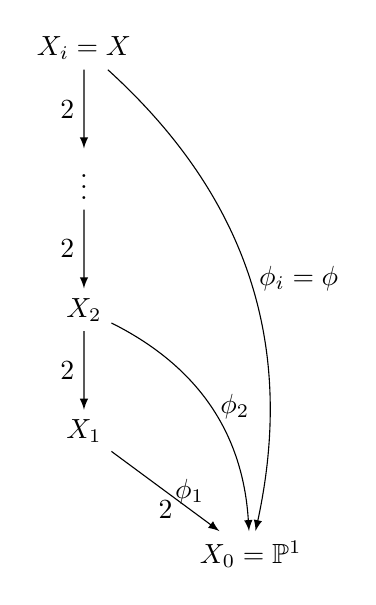
\begin{tikzpicture}[scale=0.3]
            \node at (0,0) (X0) {$X_0 = \PP^1$};
            \node [above left=of X0] (X1) {$X_1$};
            \node [above =of X1] (X2) {$X_2$};
            \node [above =of X2] (dots) {$\vdots$};
            \node [above =of dots] (Xr) {$X_i=X$};
            %\draw[<->] (X1) to node [above,rotate=-35] {$\sim$} node {} (X0);
            \draw[->] (X1) to node [below] {$2$} node [right] {$\phi_1$} (X0);
            \draw[->] (X2) to node [left] {$2$} node {} (X1);
            \draw[->, bend left] (X2) to node [below, right] {$\phi_2$} node {} (X0);
            \draw[->] (dots) to node [left] {$2$} node {} (X2);
            \draw[->] (Xr) to node [left] {$2$} node {} (dots);
            \draw[->, bend left] (Xr) to node [below, right] {$\phi_i=\phi$} node {} (X0);
            %\node at (8,0) (KX0) {$K(X_1) = K(\PP^1)$};
            %\node [above left=of KX0] (KX1) {$K(X_2)$};
            %\node [above =of KX1] (KX2) {$K(X_3)$};
            %\node [above =of KX2] (dots) {$\vdots$};
            %\node [above =of dots] (KXr) {$K(X_r)$};
            %%\draw[<->] (X1) to node [above,rotate=-35] {$\sim$} node {} (X0);
            %\draw[-] (KX1) to node [below] {$2$} node {} (KX0);
            %\draw[-] (KX2) to node [left] {$2$} node {} (KX1);
            %\draw[-, bend left] (KX2) to node [below, left] {} node {} (KX0);
            %\draw[-] (dots) to node [left] {$2$} node {} (KX2);
            %\draw[-] (KXr) to node [left] {$2$} node {} (dots);
            %\draw[-, bend left] (KXr) to node [below, left] {} node {} (KX0);
          \end{tikzpicture}
        \end{center}
        \caption{
          A $2$-group Belyi map $\phi$
          as a sequence of degree $2$ covers.
          For $j\in\{1,\dots,i\}$,
          $\phi$ factors through
          a degree $2^j$ Belyi map denoted $\phi_j$.
        }
        \label{fig:2groupfiltration}
      \end{figure}
      Let $\sigma_j$ be the permutation triple corresponding to
      $\phi_j$ in Figure \ref{fig:2groupfiltration}.
      Applying Algorithm \ref{alg:triples} to $\sigma_j$
      we obtain $\sigma_{j+1}$ as a lift of $\sigma_j$
      so that the permutation triple corresponding to $\phi$
      appears in $\mathscr{G}_{2^i}^\text{above}$.
      This shows that every $2$-group Belyi map
      of degree $2^i$ is represented by at least one node in
      $\mathscr{G}_{2^i}$.
      We now claim that every $2$-group Belyi map of degree $2^i$
      is represented by exactly one node in $\mathscr{G}_{2^i}$.
      % then show why only one in each iso class
      Since we are applying Algorithm \ref{alg:triples}
      to every permutation triple in $\mathscr{G}_{2^i}^\text{below}$,
      it is possible that in Step 2(a),
      the set of permutation triples in $\mathscr{G}_{2^i}^\text{above}$
      has simultaneously conjugate triples
      which arise when a degree $2^i$ Belyi map
      is a degree $2$ cover of more than one
      nonisomorphic Belyi map of degree $2^{i-1}$.
      In Step 2(b),
      we combine permutation triples in $\mathscr{G}_{2^i}^\text{above}$
      that are simultaneously conjugate by taking a single
      permutation triple to represent this isomorphism class
      of $2$-group Belyi map.
      Note that in Step 2(b)
      we never remove any edges in the graph
      $\mathscr{G}_{2^i}$.
      It follows from Step 2(b)
      that $\mathscr{G}_{2^i}^\text{above}$ has at most
      one node for each
      $2$-group Belyi map
      isomorphism class of degree $2^i$.
    \end{proof}
    \begin{theorem}\label{thm:isoclasses}
      The following table lists the number of isomorphism classes of
      $2$-group Belyi maps of degree $d$ for $d$ up to $256$.
      \[
        \begin{tabular}{|c||c|c|c|c|c|c|c|c|}
          \hline
          $d$ & $2$ & $4$ & $8$ & $16$ & $32$ & $64$ & $128$ & $256$\\
          \hline
          \# & $$ & $$ & $$ & $$ & $$ & $$ & $$ & $$\\
          \hline
        \end{tabular}
      \]
    \end{theorem}
    \begin{proof}
      Apply Algorithm \ref{alg:alltriples}.
    \end{proof}
    \begin{alg}\label{alg:allpassports}
      We use Algorithm \ref{alg:alltriples}
      to count the number of Passports of $2$-group Belyi maps
      of a given degree.
      \mm{todo}
    \end{alg}
    \begin{theorem}\label{thm:passports}
      The following table lists the number of passports of
      $2$-group Belyi maps of degree $d$ for $d$ up to $256$.
      \[
        \begin{tabular}{|c||c|c|c|c|c|c|c|c|}
          \hline
          $d$ & $2$ & $4$ & $8$ & $16$ & $32$ & $64$ & $128$ & $256$\\
          \hline
          \# passports & $3$ & $7$ & $16$ & $41$ & $96$ & $267$ & $834$ & $2893$\\
          \hline
        \end{tabular}
      \]
    \end{theorem}
    \begin{proof}
      Apply Algorithm \ref{alg:allpassports}.
    \end{proof}
  }
  \section{An algorithm to compute $2$-group Belyi curves and maps}{\label{sec:curvesandmaps}
    The algorithm we describe here is iterative.
    The degree $1$ case is discussed in Section \ref{sec:degree1}.
    We now set up some notation for the iteration.
    \begin{notation}\label{not:maps}
      First we suppose
      we are given the following data:
      \begin{itemize}
        \item
          $X\subset\PP^n_K$ defined over a number field $K$
          with coordinates $x_0,\dots,x_n$
          cut out by the equations $\{h_i=0\}_i$ with $h_i\in K[x_0,\dots,x_n]$
        \item
          $\phi:X\to\PP^1$ a $2$-group Belyi map of degree $d=2^n$
          given by $\phi([x_0:\dots:x_n])=[x_0:x_1]$
          with monodromy group $G = \langle\sigma\rangle$
          (necessarily a $2$-group)
          with $\sigma$ a permutation triple corresponding to $\phi$
        \item
          For $s\in\{0,1,\infty\}$ and $\tau$ a cycle of $\sigma_s\in\sigma$,
          denote the ramification point above $s$ corresponding to
          $\tau$ by $Q_{s,\tau}$
        \item
          $Y\subset\AA^n_K$ the affine patch of $X$ with $x_0\neq 0$
          with coordinates $(y_1,\dots,y_n)$ where $y_i = x_i/x_0$
          cut out by the equations $\{g_i=0\}_i$ with $g_i\in K[y_1,\dots,y_n]$
          so that $\phi:Y\to\AA^1$ is given by $\phi(y_1,\dots,y_n) = y_1$
        \item
          $\wt{\sigma}$ as in the output of Algorithm \ref{alg:triples}
          applied to the input $\sigma$
      \end{itemize}
      Algorithm \ref{alg:lift} below
      describes how to lift the degree $d$ Belyi map $\phi$
      to a degree $2d$ Belyi map $\wt{\phi}$ with ramification prescribed by $\wt{\sigma}$
      (also see Figure \ref{fig:lift}).
    \end{notation}
    \begin{figure}[ht]
      \label{fig:lift}
      \[
        \begin{tikzcd}[ampersand replacement=\&]
          \widetilde{X}\arrow{dd}[swap]{\widetilde{\phi}}\arrow{dr}{\psi}\\
          % \widetilde{X}\arrow{dd}[swap]{\widetilde{\phi}}\arrow{dr}{\text{degree 2}}\\
          \&X\arrow{dl}{\phi}\\
          \PP^1
        \end{tikzcd}
      \]
      \caption{
      Algorithm \ref{alg:lift} describes how to construct $\wt{\phi}$
        corresponding to a permutation triple $\wt{\sigma}$
        from a given $2$-group Belyi map $\phi$.
        % In Algorithm \ref{alg:lift} we construct $\wt{\phi}$
        % from a given $2$-group Belyi map $\phi$.
      }
    \end{figure}
    \begin{lemma}\label{lem:1dim}
      Let $D$ be a degree $0$ divisor on $X$.
      Then $\ddim\LL(D) \leq 1$.
    \end{lemma}
    \begin{proof}
      Suppose $\ddeg D = 0$, and
      Let $f,g\in\LL(D)\setminus\{0\}$.
      Write $D=D_0-D_\infty$ with $D_0,D_\infty\geq 0$.
      Since $f,g\in\LL(D)$, we have
      $\ddiv f,\ddiv g\geq D_0-D_\infty$.
      In particular,
      $f/g\in K^\times$.
    \end{proof}
    \begin{alg}\label{alg:lift}
      Let the notation be as described above in \ref{not:maps}.
      \newline
      \textbf{Input}: A $2$-group Belyi map $\phi:X\to\PP^1_K$
      and a permutation triple $\wt{\sigma}$
      \newline
      \textbf{Output}: A model (over $\QQal$) for the Belyi map
      $\wt{\phi}:\wt{X}\to\PP^1_K$
      with monodromy $\wt{\sigma}$
      \begin{enumerate}
        \item
          Let $R$ be the empty set of points on $X$.
          For each $s\in\{0,1,\infty\}$,
          If the order of $\sigma_s$ is strictly less than the order of $\wt{\sigma}_s$,
          then append the ramification points
          $\{Q_{s,\tau}\}_{\tau\in\sigma_s}$
          (the ramification points on $X$ above $s$ corresponding to the cycles of $\sigma_s$)
          to $R$.
        \item
          Let $D = \sum_{P}n_PP$ be a degree $0$ divisor on $X$ 
          with $n_P$ odd for every $P\in R$
          and $n_P = 0$ for $P\not\in R$.
          \mm{class group and base field}
        \item
          Compute $f\in \Kbar(X)^\times$ corresponding to a generator
          of the Riemann-Roch space $\LL(D)$.
        \item
          Write $f=a/b$ with $a,b\in \Kbar[y_1,\dots,y_n]$ and construct the ideal
          \[
            \wt{I}\colonequals\langle g_1,\dots,g_k, by_{n+1}^2-a\rangle
          \]
          in $\Kbar[y_1,\dots,y_n,y_{n+1}]$.
        \item
          Saturate $\wt{I}$ at $\langle b\rangle$ and denote this ideal by $\sat(\wt{I})$.
        \item
          Let $\wt{X}$ be the curve corresponding to $\sat(\wt{I})$ and
          $\wt{\phi}$ the map $(y_1,\dots,y_{n+1})\mapsto y_1$.
      \end{enumerate}
    \end{alg}
    \begin{proof}[Proof of correctness]
      By Algorithm \ref{alg:triples},
      there exists a $2$-group Belyi map $\wt{\phi}:\wt{X}\to\PP^1$
      with ramification according to $\wt{\sigma}$.
      Since $\wt{\phi}$ is Galois,
      the ramification behavior above each $s\in\{0,1,\infty\}$
      is constant
      (i.e. for a fixed $s$, all $Q_{s,\tau}$ are either unramified or
      ramified to order $2$).
      This ensures that the set $R$ constructed in Step $1$
      is precisely the set of ramification values of $\psi$
      (in Figure \ref{fig:lift}).
      Now that we have the ramification values,
      we can construct the new Belyi map and curve.
      We do this by extracting a square root in the function field.
      More precisely,
      again by Algorithm \ref{alg:triples},
      there exists $\wt{X}$
      with $\Kbar(\wt{X}) = \Kbar(X,\sqrt{f})$
      where $f\in\Kbar(X)^\times/\Kbar(X)^{\times 2}$
      and
      \begin{equation}\label{eqn:classgroup}
        \ddiv f= \sum_{Q_{s,\tau}\in R} Q_{s,\tau}+2D_\epsilon
        \in\frac{\Div^0(X)}{2\Div^0(X)}
      \end{equation}
    \end{proof}
    \begin{example}
    \end{example}
  }
  \section{Running time analysis}{\label{sec:runtime}
  }
  \section{Explicit computations}{\label{sec:computations}
  }
} 
\chapter{Results on $2$-group Belyi maps}{\label{chapter:results}
  In this chapter we discuss some results on $2$-group Belyi maps
  obtained, in part, from the data in
  Chapter \ref{chapter:database}.
  Section \ref{sec:classification} details which types of Belyi maps
  can occur as $2$-group Belyi maps.
  Section \ref{sec:fieldsofdefinition} describes the possible
  fields of definition
  and fields of moduli for $2$-group Belyi maps.
  \section{Classifying $2$-group Belyi maps}{\label{sec:classification}
    The conditions that need to be satisfied for a general Belyi map
    to be a $2$-group Belyi map are quite stringent.
    For example,
    the ramification indices can be encoded as a triple of integers
    $(a,b,c)\in\{1,2,4,\dots\}^3$.
    We start Section \ref{sec:classification} by giving a complete description of the geometry type
    (see Definition \ref{def:geometrytype}) of a
    $2$-group Belyi map in Proposition \ref{prop:geometrytype}
    and finish Section \ref{sec:classification}
    with a classification of hyperelliptic
    $2$-group Belyi maps in Theorem \ref{thm:hyperelliptic}.
    \begin{prop}\label{prop:geometrytype}
      Let $\phi:X\to\PP^1$ be a $2$-group Belyi map
      corresponding to a permutation triple $\sigma$
      with $(a,b,c)$ the triple of orders of permutations in $\sigma$.
      Then the geometry type of $\phi$ is determined by $(a,b,c)$
      and is one of the following:
      \begin{enumerate}
        \item[(degenerate)]
          $\phi$ is degenerate if $1\in(a,b,c)$.
        \item[(spherical)]
          $\phi$ is spherical if $(a,b,c)$ is of the form
          $(2,2,c)$, $(2,b,2)$, or $(a,2,2)$.
        \item[(Euclidean)]
          $\phi$ is Euclidean if $(a,b,c)$ is of the form
          $(2,4,4)$, $(4,2,4)$, or $(4,4,2)$.
        \item[(hyperbolic)]
          $\phi$ is hyperbolic (with genus at least $2$) in all other cases.
      \end{enumerate}
    \end{prop}
    \begin{proof}
    \end{proof}
    \subsection{Classifying spherical $2$-group Belyi maps}{\label{subsec:elliptic}}{
    }
    \subsection{Classifying genus $1$ $2$-group Belyi maps}{\label{subsec:elliptic}}{
    }
    \subsection{Classifying hyperelliptic $2$-group Belyi maps}{\label{subsec:hyperelliptic}}{
      \begin{definition}
        Let $K$ be a number field with algebraic closure $\overline{K}$.
        Let $X$ be an irreducible smooth projective curve over $K$.
        $X$ is \defi{hyperelliptic} if there exists a degree $2$ morphism
        $\iota:X\to\PP^1$ (defined over $\overline{K}$).
        The degree $2$ morphism $\iota$ is called the
        \defi{hyperelliptic involution}.
      \end{definition}
      \begin{definition}
        A \defi{hyperelliptic Belyi map} is a Belyi map $\phi:X\to\PP^1$
        where $X$ is a hyperelliptic curve.
      \end{definition}
      \begin{lemma}\label{lem:hyperellipticinvolution}
        Let $\phi:X\to\PP^1$ be a hyperelliptic $2$-group Belyi map
        with monodromy group $G$.
        Let $\iota$ denote the hyperelliptic involution in $\Aut(X)$.
        Then
        $G\leq\Aut(X)$ and $\iota$ is central in $G$.
      \end{lemma}
      \begin{proof}
      \end{proof}
      \begin{theorem}\label{thm:hyperelliptic}
        Let $\phi:X\to\PP^1$ be a hyperelliptic $2$-group Belyi map
        with monodromy group $G$.
        Let $\iota$ denote the hyperelliptic involution in $\Aut(X)$.
        Then $\overline{G}\colonequals G/\langle\iota\rangle$
        is a subgroup of $\Aut(\PP^1)\cong\PGL_2(\CC)$.
        (see Figure \ref{fig:hyperelliptic}).
        In particular,
        $\overline{G}$ is either cyclic, dihedral, or exceptional.
        \begin{figure}[ht]
          \[
            \begin{tikzcd}[ampersand replacement=\&]
              X\arrow{dd}[swap]{G}\arrow{dr}{\langle\iota\rangle}\\
              \&\PP^1\arrow{dl}{G/\langle\iota\rangle}\\
              \PP^1
            \end{tikzcd}
          \]
          \caption{
            A hyperelliptic $2$-group Belyi map
            with monodromy group $G$
            factors through a degree $2$ map to $\PP^1$
            and an automorphism of $\PP^1$.
          }
          \label{fig:hyperelliptic}
        \end{figure}
      \end{theorem}
      \begin{proof}
      \end{proof}
    }
  }
  \section{Fields of definition of $2$-group Belyi maps}{\label{sec:fieldsofdefinition}
    In Section \ref{sec:fieldsofdefinition} we use the data
    from Chapter \ref{chapter:database} to 
    formulate a conjecture about the possible fields of definition of
    $2$-group Belyi maps.
    Recall the action of $G_\QQ$ on the set of Belyi maps
    described in Proposition \ref{prop:galoisaction}.
    For a fixed Belyi map,
    we can simplify matters as described in the following definition.
    \begin{definition}\label{def:fieldofmoduli}
      The \defi{field of moduli} of a Belyi map
      $\phi:X\to\PP^1$ is the fixed field
      \[
        \{\tau\in G_\QQ : \phi^\tau\cong\phi\}.
      \]
    \end{definition}
    Definition \ref{def:fieldofmoduli} allows us to study
    a more manageable finite extension.
    Moreover, passports (recall Definition \ref{def:passport})
    allow us to bound the degree of the field of moduli.
    \begin{theorem}\label{thm:fieldofmoduli}
      Let $\phi:X\to\PP^1$ be a Belyi map
      with passport $\mathcal{P}$.
      Then the degree of the field of moduli of $\phi$
      is bounded by the size of $\mathcal{P}$.
    \end{theorem}
    \begin{proof}
      % proof in JVSijsling
    \end{proof}
    \begin{definition}\label{def:refined}
      A \defi{refined passport} $\mathcal{P}$ consists of the data
      $(g,G,C)$
      where $g\geq 0$ is an integer,
      $G\leq S_d$ is a transitive subgroup,
      and $C = (C_0,C_1,C_\infty)$
      is a triple of conjugacy classes of $G$.
    \end{definition}
    \mm{some exposition about refined passports}
    For a refined passport $\mathcal{P}$ consider the set
    \[
      \Sigma_\mathcal{P} =
      \{(\sigma_0,\sigma_1,\sigma_\infty)\in C_0\times C_1\times C_\infty : \sigma_\infty\sigma_1\sigma_0=1,\text{ and } \langle\sigma\rangle=G\}/\sim
    \]
    where $(\sigma_0,\sigma_1,\sigma_\infty)\sim(\sigma_0', \sigma_1', \sigma_\infty')$
    if and only if there exists $\alpha\in\Aut(G)$ with
    $\alpha(\sigma_s) = \sigma_s'$ for $s\in\{0,1,\infty\}$.
    \begin{conj}
      Let $\mathcal{P} = (g,G,C)$
      be a refined passport with
      $G=\Mon(\phi)$ for some $2$-group Belyi map $\phi$.
      Then $\#\Sigma_\mathcal{P} = 0\text{ or }1$.
    \end{conj}
    \begin{proof}
    \end{proof}
    \begin{corr}
      Every $2$-group Belyi map is defined over a cyclotomic field
      $\QQ(\zeta_{2^m})$ for some $m$.
    \end{corr}
    \begin{proof}
    \end{proof}
  }
}
\chapter{Gross's conjecture for $p=2$}{\label{chapter:grossconjecture}
  We begin this chapter with Theorem \ref{thm:beckmann} which provides
  the arithmetic motivation to study $2$-group Belyi maps.
  We then detail past results on Gross's conjecture in Section
  \ref{sec:grossconjecturepast}
  and finish with some discussion on $2$-group Belyi maps
  in relation to the $p=2$ case of Gross's conjecture.
  \section{Beckmann's theorem}{\label{sec:beckmann}
    In this Section we state Beckmann's theorem
    for Belyi maps over $\CC$
    from
    $1989$ which can be found in \cite{beckmann}.
    We then adapt Theorem \ref{thm:beckmann}
    to our particular situation in
    Corollary \ref{cor:beckmann}.
    \begin{theorem}\label{thm:beckmann}
      Let $\phi:X\to\PP^1$ be a Belyi map with
      monodromy group $G$
      and suppose $p$ does not divide $\# G$.
      Then there exists a number field $M$
      with the following properties:
      \begin{itemize}
        \item
          $p$ is unramified in $M$
        \item
          the Belyi map $\phi$ is defined over $M$
        \item
          the Belyi curve $X$ is defined over $M$
        \item
          $X$ has good reduction at all primes $\mathfrak{p}$
          of $M$ above $p$
      \end{itemize}
    \end{theorem}
    \begin{proof}
      \cite{beckmann}
    \end{proof}
    \begin{corr}\label{cor:beckmann}
      Let $\phi:X\to\PP^1$ be a $2$-group Belyi map.
      Then there exists a smooth projective model for $X$
      with good reduction away from $p=2$.
    \end{corr}
    \begin{proof}
    \end{proof}
  }
  \section{Past results on Gross's conjecture}{\label{sec:grossconjecturepast}
  }
  \section{A nonsolvable Galois number field ramified only at $2$}{\label{sec:numberfieldramifiedat2}
  }
}

%%%%%%%%%%%%%%%%%%%%%%%%%%%%%%%%%%%%%%%%%%%%%%%%%%
%Backend of thesis (references and the like)
%%%%%%%%%%%%%%%%%%%%%%%%%%%%%%%%%%%%%%%%%%%%%%%%%%
\backmatter

%Add your bibliography filename and uncomment these lines
\bibliographystyle{amsplain}
\addcontentsline{toc}{chapter}{References}
\bibliography{references}

%Uncomment if you want an index
%\printindex

\end{document}
